\documentclass[a4paper,10pt]{article}
\usepackage[english]{babel}
\usepackage{thesis}
%\usepackage{a4wide}
% Small enumerate and itemize
\usepackage{mdwlist}

% Fill in the header:
\lhead{Combining Robocup Rescue and XABSL}
\rhead{Maarten de Waard}

\begin{document}

\begin{center}
\thispagestyle{empty}


\vspace{2.5cm}

% [CHANGE] The title of your thesis. If your thesis has a subtitle, then this
% should appear right below the main title, in a smaller font.
\hrulefill\\
\begin{Huge}
Bachelor project: Midterm report\\
\end{Huge}
\vspace{0.2cm}
\begin{Large} 
Combining Robocup Rescue and Xabsl\\
\end{Large}
\hrulefill\\
\vspace{0.5cm}

\includegraphics[width=\textwidth]{uva.jpg}
\vspace{0.5cm}

% [CHANGE] Your full name. In case of multiple names, you can include their
% initials as well, e.g. "Jan G.J. van der Wegge".
{
\Large
Maarten P. de Waard\\\vspace{0.2cm}
% [CHANGE] Your student ID, as this has been assigned to you by the UvA
% administration.
\textit{5894883}
}

\vspace{1.5cm}

% [DO NOT CHANGE]
Bachelor thesis\\
% [CHANGE] Whether your Bachelor thesis is 6 ECTS (regular) or 9 ECTS (Honours
% programme).
Credits: 6 EC

\vspace{0.5cm}

% [DO NOT CHANGE] The name of the educational programme.
Bsc. Artificial Intelligence

\vspace{0.25cm}

% [DO NOT CHANGE] The addess of the educational programme.
University of Amsterdam\\
Faculty of Science\\
Science Park 904\\
1098 XH Amsterdam

\vspace{2cm}

\emph{Supervisor}\\
% [CHANGE] The name of your supervisor. Include the titles of your supervisor,
% as well as the initials for *all* of his/her first names.
dr. A. Visser 

\vspace{0.25cm}

% [CHANGE] The address of the institute at which your supervisor is working.
% Be sure to include (1) institute (is appropriate), (2) faculty (if
% appropriate), (3) organisation name, (4) organisation address (2 lines).
Informatics Institute\\
Faculty of Science\\
University of Amsterdam\\
Science Park 904\\
1098 XH Amsterdam\\

\vspace{1.5cm}

% [CHANGE] The date at which you will finalize and submit your thesis.
June 26th, 2012

\end{center}
\newpage


\begin{abstract}
In this research, a product will be introduced, that combines the Extensible
Agent Behavior Specification Language (XABSL) with any program, capable of
having a socket connection. A use of this product is shown, by combining it to
the rescue project on the University of Amsterdam, using
\textit{UsarCommander},
a program designed to control one or more robots, in a virtual rescue operation.
\end{abstract}
%\begin{multicols}{2}
\section{Introduction}
The research will be focussing on combining the \textit{Extensible Agent
Behavior Specification Language} (XABSL) with any program capable of making a
socket connection. In particular, the focus will lay on virtual rescue
operations, otherwise known as the \textit{RoboCup Rescue League}. Using a
behavior specification language will make it possible to separate specification
of behaviors from implementation.

Currently, the focus of research in the rescue missions is mainly on creating
smart implementations of sensors. Much of the actual controlling of robots is
done by hand, using programs that forward the camera images of the robots to a
human operator controlling them. Some of these operators use simple behaviors to
help them, like for example making the robot automatically traverse a path to a
specified point. This kind of simple task can be called a behavior.

An improvement that can be made in these behavior controlled robots, is in 
the specification of which behavior should be selected in a certain situation
and how the behavior is executed. This can be done by creating
behavior-controlled robots, that can autonomously select the best behavior to
activate on a certain moment, and using their sensors as input, can choose the
right way to navigate.

This research will make use of XABSL, a behavior specification language, which
makes it possible to separate the specification of a behavior, from the implementation.

%Results in the RoboCup Rescue missions are counted by how many victims
%are found on the map, so improvement can be shown by finding more victims using
%the results of this research.
%

Currently, not many behavior-controlled exploration algorithms exist.
An exception is path finding on challenging terrain
\cite{seraji2002behavior} . This research will result in a method to
easily adjust and improve the behavior of any robot in any robot commanding
program, especially focussing on UsarCommander, the program used by the UvA Rescue
team\footnote{Team description and more at: \url{http://www.jointrescueforces.eu/wiki/tiki-index.php}}.

There has however been research in Behavior Based Artificial Intelligence since
1986.

\section{Behavior Based Artificial Intelligence}
This was first researched by brooks \cite{brooks1986robust}, who laid the
foundations of looking at intelligence in different layers. Brooks proposed that
the following four elements were key requirements in a robot controlling system:
\begin{enumerate}
    \item \textbf{Multiple goals:} A robot should be able to chase multiple goals at the
    same time, for example reaching a place in minimal time, while conserving
    power reserves. There should be an ability to prioritize goals, so that
    dangerous situations can be evaded while the main goals are still executed
    when the robot is able to. A simple example is being able to evade obstacles
    while reaching the place it wants to reach.
    \item \textbf{Multiple sensors:} Most robots have more than one sensor, each
    having its own error measure. Some sensors have a bigger error in certain
    situations then others. For example while traversing inside a building, a
    robot should not be trusting its GPS sensor (Global Positioning Satelite),
    while being outside this would be a good option. A robot should be able to
    cope with these different errors, and use the right sensors at the right
    time with the right amount of trust.
    \item \textbf{Robustness:} A robot's artificial intelligence should be
    robust. This means that when certain sensors fail, or unexpected
    deviations from it's normal environment occur (for example when a robot for
    inside-use comes outside a building, where there are less walls, but more
    smaller obstacles), the robot should still be able to act in a sensible way,
    in stead of just stop and stay still, or act randomly.
    \item \textbf{Extensibility:} Brooks only speaks of being able to enlarge
    the processing power of the robot, when more sensors are loaded on the
    robot. I would like to add to this, that the intelligent system should have
    some kind of modularity in its software, making extending the system to work with a new kind
    of sensor, or even a totally different robot or environment (for example
    virtual vs the real world) easy, without having to rewrite big parts of
    code, or search through the program to find where a sensor should be added
    and where the activation of the sensor occurs, etc.
\end{enumerate}

Brooks explains that typically, robot intelligences slice problems up in the
following order: Sense, map sensor data in a world representation, plan, execute
task and at last: control motors to do so. He then offers a new implementation
of problem-decomposing, in the following order, and calls these `Levels of
competence'

\begin{enumerate*}
\setcounter{enumi}{-1}
\item ``Avoid contact with objects (whether the objects move or
are stationary).''
\item ``Wander aimlessly around without hitting things.''
\item ```Explore' the world by seeing places in the distance
that look reachable and heading for them.''
\item ``Build a map of the environment and plan routes from one
place to another.''
\item ``Notice changes in the `static' environment.''
\item ``Reason about the world in terms of identifiable objects
and perform tasks related to certain objects.''
\item ``Formulate and execute plans that involve changing the
state of the world in some desirable way.''
\item ``Reason about the behavior of objects in the world and
modify plans accordingly.''
\end{enumerate*}

\begin{figure}
    \centering
    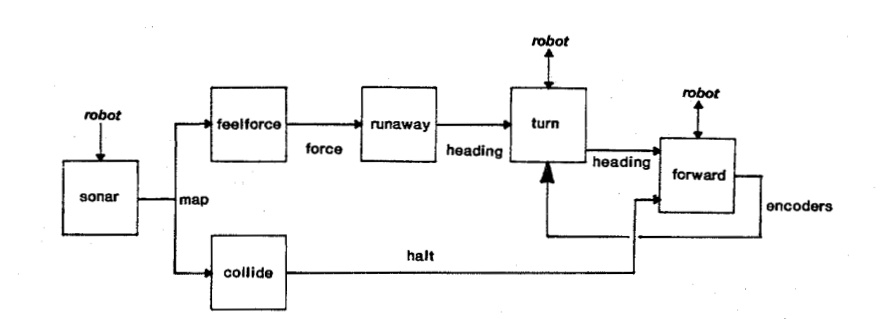
\includegraphics[width=.8\textwidth]{images/level0.png}
    \label{fig:levelzero}
    \caption{A level 0 control system, as proposed by Brooks}
\end{figure}
\begin{figure}
    \centering
    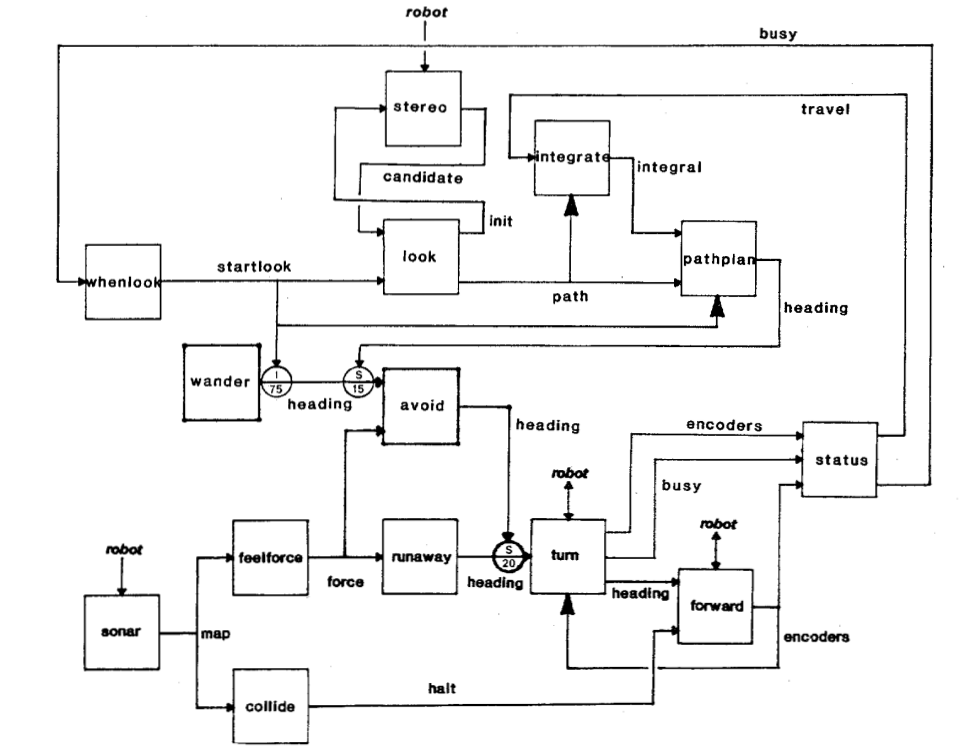
\includegraphics[width=.8\textwidth]{images/level2.png}
    \label{fig:leveltwo}
    \caption{A level 2 control system, as proposed by Brooks}
\end{figure}

Each level of competence adds complexity to the entire system, thereby creating
a layered implementation of behavior in an (in that time) untraditional way.
Brooks proposes that each of these layers can be implemented in a finite state
automaton, resulting in figure \ref{fig:levelzero} as a representation for the
zeroth level, and, by augmenting this with an FSA for level one and two, in
figure \ref{fig:leveltwo}.

In the level 0 representation, the robot will `run away' when it is standing
still and a moving object closes in. Alternatively, it will halt when a probable
collision is detected. This is enough for simple obstacle avoidance.

This representation is augmented by inserting the avoidance and wander states
above it parallel to the runaway state, in figure \ref{fig:leveltwo},
This results in level 1 behavior: a robot capable of
wandering around aimlessly, without hitting any objects. The direction outputted
by the level 0 FSA is, when possible, overridden by the direction of the level 1
output. 

As can be seen, this method a very large FSA, when we add the second level of
control. This has the advantage of being capable of more complex behavior, in
this case exploring an area, thus no more simply wandering around, but reaching
places it has not yet explored. A disadvantage of this method, however, is that
these big FSA's are quite complex to understand Adding more and more complexity
to the system results in bigger and bigger images, resulting in more
representation complexity and, in the worst case, in a system that only the
creator can understand fully, but cannot anymore be represented in a clear way.
Of course it needs to be considered that this system was created in 1986, when
computers were many times slower and capabilities were limited. Brooks managed
to get the level 2 version working on a real robot in the time, by distributing
the system over many cores.

This is the main advantage Brooks proposes, of this kind of implementation: The
processes needed for the in- and output of the states, can be done with the
least possible interaction between processes, making Brooks able to distribute
the implementation over different processors and thereby able to run this, for
that time, complex program.

Nowadays, this implementation is a bit outdated, mainly because of the complex
structure of the representation. The behavior based approach, however, has been
used in several solutions to controlling robots. These solutions will be
discussed in the following section.

\section{BBAI Implementations and Alternatives}
This section will cover most of the BBAI implementations that can be chosen from
when deciding to create an application that should be capable of specifying a
Behavior Based artificial intelligence. 

\subsection{XABSL}
One of the implementations of behavior based software is \textit{XABSL}: a
 programming language, created to easily describe behaviors for autonomous agents
based on hierarchical finite state machines \cite{loetzsch2003xabsl}. It is the
software that has been used by the German robotic soccer team to specify their
robots' behaviors. The team won in 2008, and the years after that.

The language is used to specify a finite state automaton hierarchy. This means
that the user defines several finite state automata, which can activate each
other. Each state makes decisions on certain variables, and as an output
activate another state or another FSA. The hierarchies are built up from the
following components:

\begin{figure}
    \centering
        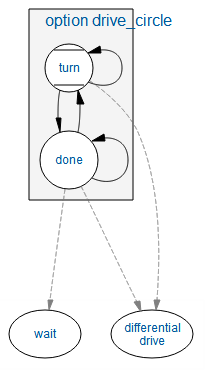
\includegraphics[height=5cm]{../files/option_drive_circle.png}
        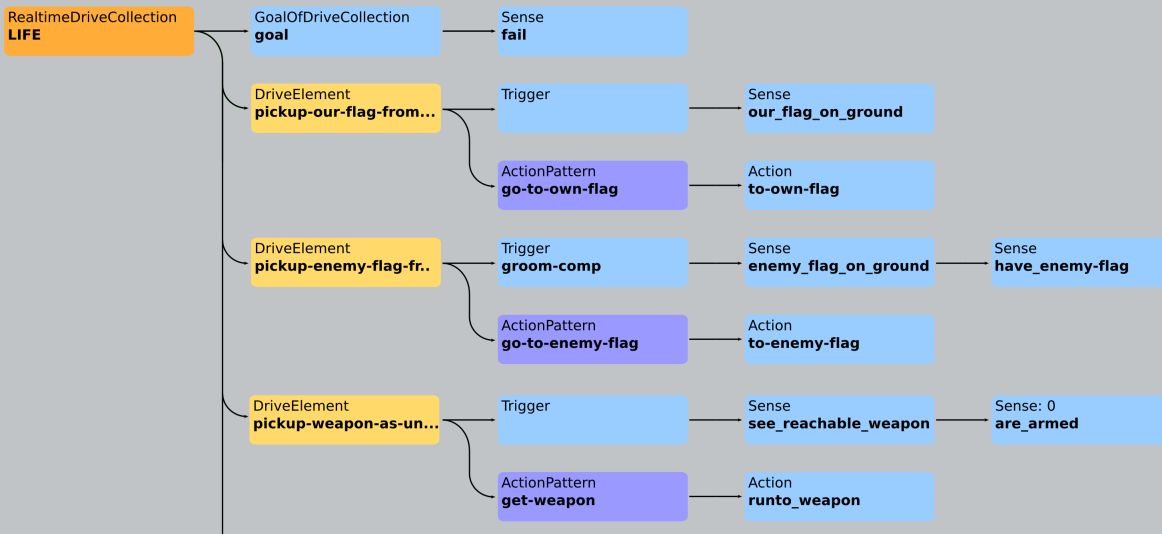
\includegraphics[height=5cm]{images/POSH-smaller.png}
    \label{fig:simpleFsm}
    \caption[XABSL hierarchy and POSH hierarchy]{Left: An example of a figure generated by the XABSL compiler, from
    XABSL code. Right: a POSH hierarchy}
\end{figure}
A XABSL-specification is built up from the following components:

\begin{itemize}
\item \emph{Agents:} A rooted acyclic graph, containing all the behaviors for one
agent. Several of these agents can be created, all having their own graph and
thus their own behavior.
\item \emph{Options:} Complex agent behavior. Each option is on itself a finite
state machine, containing several states. When creating an agent, the start
option can be specified, which makes the user able to create different agents
from one Option hierarchy. Options can also have parameters, enabling an option
to have different outputs for different agents. Figure \ref{fig:simpleFsm}
contains an example of a simple option, that makes the agent turn 360 degrees
and then stop and wait for a certain amount of time.
\item \emph{States:} Options are bounded to each other by states, each state has
a decision tree, and an action. The decision tree decides whether to stay at
this state, or to go to another state. These decisions are based on variables
that can either be internal, or inputs.

When a decision tree decides to stay at its current state, an action is
performed. Actions can be activation of a basic behavior, or of another option.
Several actions per state are permitted.
\item \emph{Basic behavior:} At every leaf of an option (so, every state with no
other states to reference to) a basic behavior is activated. This is a small
piece of native code (C++ or Java), that influences the actions of the agent
in its world. 
\end{itemize}

This is an improvement over Brooks' BBAI, because the FSA's are now no
longer directly connected to each other through state connections, but are
connected via the actions of
certain states, in that way improving the comprehensibility of the
representation, thereby also improving the modularity of the system, because
modules can be better recognized and then expanded.

By using basic behaviors, that can be written in C++ or Java, XABSL also
enables distribution of the system: Each basic behavior can run its own module.
This way basic behavior can be a module that simply makes a robot move, but also a
module that finds a ball in a soccer field, using libraries like OpenCV. This
makes a XABSL application capable of the same things as any native C++ or Java
application, which is almost everything one or more computers can do.

Section \ref{sec:xabsl-focus} will explain more clearly the advantages of XABSL,
and the possibilities of agents, options, states and basic behaviors.

\subsection{POSH}
POSH \cite{brom2006posh} is a very similar alternative implementation of a Behavior Specification
Language. Posh is defined as a \textit{Behavior Oriented Design}, which is
a combination of \textit{Object Oriented Design} (OOD, used by object oriented
programming languages like Java and C++) and \textit{Behavior Based Artificial
Intelligence} (BBAI). 

From OOD the language takes the object hierarchy that it is known for. In object
oriented languages a person is capable of creating an object based on another
object. These can be \textit{Abstract classes}, or \textit{Interface classes}. When using an
abstract class to define an object, this means the class can be extended by
another object: The new object automatically has all the properties its
\textit{Base class} (the original, abstract, class) has, but can override some
of them, or add new ones. An interface class can define what its subclass should
have, for example when an interface class specifies a method that searches for a
doorway, using laser sensors, its subclass should implement this method. The
interface class itself does not have any actual implementations. BOD objects are literally built in an object oriented language, thereby having
all its advantages

The BBAI-part of it is the decomposition of intelligence
as subtasks called \textit{acts}. Examples of acts are knowing your position and
planning a route. There is no implementation of prioritizing certain acts above
others, other than that they come earlier in the POSH diagram. 

Behaviors in BOD are thus specified as a \textit{Behavior object}, written in an
Object Oriented language. They are split up in actuators and senses. The
actuators are used to act on the world, for example move in a certain direction,
or pick something up, whereas the senses are used to inform the planner the
current context. Context can be any piece of information about the world, or the
agents internal state. The
whereabouts of an object, or the data from a laser scanner can be context, but
the agents current battery level is also context.. All the specified behaviors together form the
\textit{Behavior Library}, which can be used by the action planning system to
select the right behavior on the right time. 

Furthermore POSH uses three aggregates: simple sequences, competences and drive
collections.

\begin{enumerate}
    \item \textbf{Simple sequences:}
        The sequence is simply a sequence in which order a diagram should be
        traversed
    \item \textbf{Competences:}
        A competence is a prioritised set of condition-action pairs. These
        condition-action pairs are based on the current context (described
        above). Because of the hierarchical structure of the system, only small
        pieces of context have to be processed at a time. When a certain part of
        competence is reached, competences have been passed higher up in the
        hierarchy, meaning that this information needs no more checking. In this
        part there is assumed that in the time it took to traverse the tree, the
        world has not changed significantly.
    \item \textbf{Drive Collections:}
        The drive collection is a special competence, that is executed before
        each program cycle. The collection contains all vital condition-action
        pairs to be able to survive. For example when an enemy is close (given
        that the environment has enemies that can seriously harm the agent), the
        agent should hide from the enemy, or take other actions not to get
        harmed. The drive collection can also contain routines that have to be
        executed every once in a while, like checking the environment for safety
\end{enumerate}

This is actually quite similar to XABSL,
because selects actions based on decisions based on its findings. 
The actions are always executed by an external program. There are some important differences though:

\begin{itemize}
    \item POSH is designed to be used by non-pro\-gram\-mers. This means the
    interface is easy, colorful and simple, whereas XABSL prioritizes complex
    capabilities, ignoring the fact that non-programmers then couldn't use it.
    This improves the adaptability of XABSL far above the capabilities of POSH,
    resulting in ability to create more complex behaviors.
    \item Where XABSL has a close coupling with the perception stream of the
    robot, POSH has no variable management, enabling the system to be a lot
    easier to use, but also maximizing the complexity of the specified behaviors
    to a lower maximum than XABSL offers.
\end{itemize}

\subsection{Petri Net Plans}
% First describe petri nets
Another possible method to represent robot behavior as plans, is by using
\textit{Petri Net Plans}. This is a language based on \textit{Petri Nets} (Also known as
Place/Transition Nets or P/T Nets), proposed by \cite{ziparo2011petri}. 

Before going into the petri nets, it is useful to know what a Petri Net exactly
is. 

\subsection{COLBERT}
\cite{konolige1997colbert}

These are the main alternatives. There are others, like using constraint logic,
with aid of If-then-else statements directly in the main program. One can also
use machine learning techniques, for example \textit{Reincorcement Learning}
methods are used by \textit{Sarsa} and \textit{Q-learning}. This is, however a
complete different way of looking at the problem, with its own set of results,
which are not comparable to the ones reachable with human-specified behaviors,
because the current learning techniques are not yet sufficient.

\subsection{XABSL specification}
XABSL makes use of four components: Agents, Options, states and Basic behavior.
The following subsections will explain what these are, and how they can be used.

\subsection{Agents}
An XABSL agent is a rooted acyclic graph, containing all the behaviors for one
agent. In this research, one agent will equal one robot. 






\subsubsection{Motivation to use it}
Using FSM's for behavior is an easily comprehensible method to specify behavior.
The advantages of XABSL are that tools are delivered to make a hierarchy
documentation for your website (or anything else). For example, the FSM in
figure \ref{fig:simpleFsm} is automatically generated from XABSL code.

Using this representation, tweaking the behavior should become an easier task
resulting in better results for autonomous exploration.

% TODO
This section will be expanded with the following: 

\section{RoboCup Rescue}
\subsection{Description}
The project used in cooperation with the application, is UsarCommander.
UsarCommander\footnote{Available at
\url{http://www.jointrescueforces.eu/wiki/tiki-index.php}}, originally developed by Bayu Slamet, and extended by Arnoud
Visser and many others. This program takes care of connecting to USARSim (the
simulator used in the Robocup) and
makes the user able to easily get sensor data from the robots in it. It is also
possible to control the robots with several types of behavior, like
corridor-following, obstacle-avoidance, or tele-operation. The last of which
enables the operator to manually control the robots by hand, using an
interactive human interface.

Over time, the system has been expanded with many subprojects, for example one
implementing a SLAM
(Simultaneous Localisation And Mapping) algorithm, to make an accurate map from
the sensor data of several robots\cite{slamet2006manifoldslam}. All the information used and produced by
these subprojects can be accessed by other subprojects, resulting in an ideal
environment for creating new robot-controlling applications.

\subsection{Motivation to use it}
The main reason to use this program, instead of any other, to interface my
software with USARSim is that it has so many features. The presence of many
subprojects in the code, makes it possible to make a very efficient autonomous
exploration algorithm interfacing with the subprojects at hand. Without using UsarCommander all
the needed software should be taken from somewhere else, or implemented solely
for this purpose.

Other software for this purpose is available too. %TODO: Specify other programs

but since this is a bachelor
thesis on the University of Amsterdam, and this is the software used by it in
the RoboCup, this is the logical choice.
\section{Approach}
\begin{comment}
This section will contain my approach
\end{comment}

\subsection{Interfacing both programs}
Since the UsarCommander is written in Visual Basic, and the basic behaviors of
XABSL are written in C++, a bridge should be made. This is done by creating a
Dynamic Link Library (DLL). This DLL contains the needed functions of the C++
program, making them accessible for Visual Basic. The bridge works both ways, so
Visual Basic can offer output symbols to the XABSL Engine, while the engine can
offer input symbols to the agent.

\subsection{Creating a succesful hierarchy}
This section will tell about the FSM hierarchy I will make for autonomous
exploration


\section{Results}
This section will contain results, hopefully in the form of explored maps, numbers of victims found, etc.

\section{Conclusion}

%\end{multicols}{2}
\bibliography{bib}{}
\bibliographystyle{plain}
\end{document}

